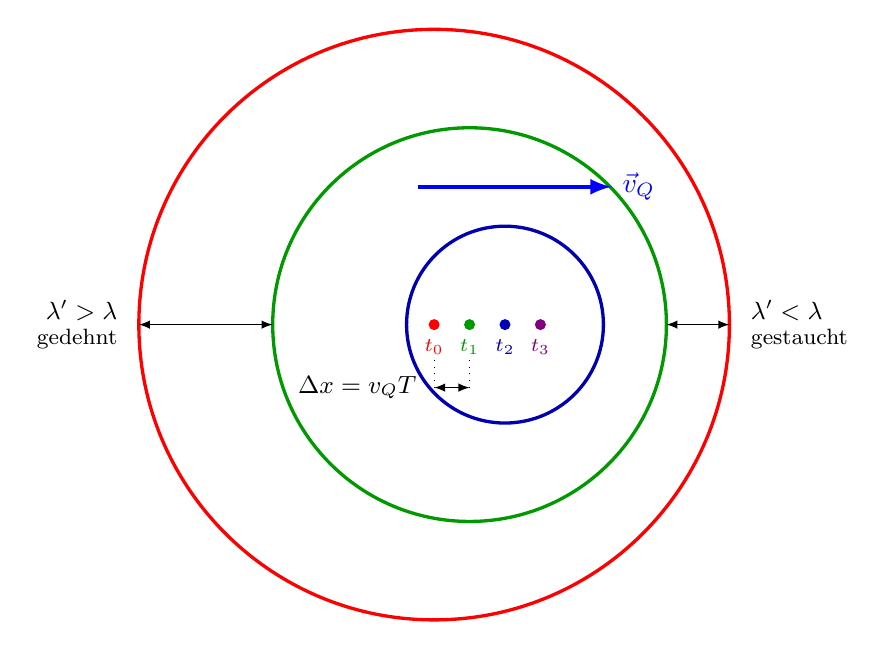
\begin{tikzpicture}[>=latex, scale=1]
  \def\ut{1.25}   % u*T in cm
  \def\dx{0.45}   % v_Q*T in cm  (v_Q = 0.36 u)
  % Kreise: Welle, ausgesendet bei t0 (r=3uT), t1 (2uT), t2 (uT), t3 (0)
  \draw[red,   very thick] (0*\dx,0) circle (3*\ut);
  \draw[green!60!black, very thick] (1*\dx,0) circle (2*\ut);
  \draw[blue!70!black,  very thick] (2*\dx,0) circle (1*\ut);
  % Quellenpositionen
  \foreach \i/\c in {0/red,1/green!60!black,2/blue!70!black,3/violet}{
    \fill[\c] (\i*\dx,0) circle (0.07);
  }
  \node[below=2pt, font=\scriptsize, red] at (0,0) {$t_0$};
  \node[below=2pt, font=\scriptsize, green!60!black] at (\dx,0) {$t_1$};
  \node[below=2pt, font=\scriptsize, blue!70!black] at (2*\dx,0) {$t_2$};
  \node[below=2pt, font=\scriptsize, violet] at (3*\dx,0) {$t_3$};
  % Geschwindigkeit
  \draw[->, ultra thick, blue] (-0.2,1.75) -- (3*\dx+0.9,1.75) node[right] {$\vec v_Q$};
  % Delta x
  \draw[<->] (0,-0.8) -- (\dx,-0.8);
  \draw[dotted] (0,-0.45) -- (0,-0.85); \draw[dotted] (\dx,-0.45) -- (\dx,-0.85);
  \node[left, font=\small] at (-0.1,-0.8) {$\Delta x = v_Q T$};
  % Wellenlaenge vor / hinter der Quelle
  \draw[<->] (2*\ut+\dx,0) -- (3*\ut,0);
  \draw[<->] (-3*\ut,0) -- (-2*\ut+\dx,0);
  \node[right, font=\small, align=left] at (3*\ut+0.15,0) {$\lambda'<\lambda$\\[-2pt]\footnotesize gestaucht};
  \node[left, font=\small, align=right] at (-3*\ut-0.15,0) {$\lambda'>\lambda$\\[-2pt]\footnotesize gedehnt};
\end{tikzpicture}
